%!TEX TS-program = xelatex
% !Mode:: "TeX:UTF-8"
\documentclass[a4paper]{ctexart}%{article}
\usepackage[margin=2cm]{geometry}
\usepackage{amsmath,amssymb,amsthm}
\usepackage[inline]{enumitem}
\renewcommand{\baselinestretch}{1.67}
\pagestyle{empty}

\usepackage{xeCJK}
            \newCJKfontfamily\Kaiti{Adobe Kaiti Std}
            \newCJKfontfamily\Heiti{Adobe Heiti Std}
\setCJKmainfont[BoldFont={Adobe Heiti Std},ItalicFont={Adobe Kaiti Std}]{Adobe Song Std} % 粗体与斜体的替代

%            \newcommand{\sanhao}{\fontsize{16.1pt}{\baselineskip}\selectfont}    % 三号
%            \newcommand{\sihao}{\fontsize{14.1pt}{\baselineskip}\selectfont}        % 四号
\punctstyle{kaiming}

\usepackage{tikz}

%\usepackage{picinpar}    % picinpar 是用来调整图片位置
\usepackage{esvect}       %向量\vv
\usepackage{stmaryrd}  %平行\sslash

%%%%%%%%%%%%%%%%%%%%%%%%%%%%%%%%%%%%%%%%%%%%%%%%%%%%%%%%
%%%%%%%%%%%%%%%%%%%%%%%%%%%%%%%%%%%%%%%%%%%%%%%%%%%%%%%%

\newfontfamily\CM{Cambria Math}                                                                                          %编号圈1 到圈10
\newcommand{\cmcirc}[1]{\pgfmathparse{
                ifthenelse(#1 > 0 && #1 < 21, Hex(9311+#1), Hex(9450))
                }{\CM{\symbol{"\pgfmathresult}}}}
\newcommand{\cmcircblk}[1]{\pgfmathparse{
                ifthenelse(#1 > 0 && #1 < 11, Hex(10101+#1),
                                       ifthenelse(#1 > 10 && #1 < 21, Hex(9450-10+#1),
                                                                           Hex(9471))
                                      )
                }{\CM{\symbol{"\pgfmathresult}}}}


%%%%%%%%%%%%%%%%%%%%%%%%%%%%%%%%%%%%%%%%%%%%%%%%%%%%%%%%
%%%%%%%%%%%%%%%%%%%%%%%%%%%%%%%%%%%%%%%%%%%%%%%%%%%%%%%%

\makeatletter                   %直立\pi
 \newcommand{\allmodesymb}[2]{\relax\ifmmode{\mathchoice
 {\mbox{\fontsize{\tf@size}{\tf@size}#1{#2}}}
 {\mbox{\fontsize{\tf@size}{\tf@size}#1{#2}}}
 {\mbox{\fontsize{\sf@size}{\sf@size}#1{#2}}}
 {\mbox{\fontsize{\ssf@size}{\ssf@size}#1{#2}}}}
 \else
 \mbox{#1{#2}}\fi}
 \makeatother

 \newfontfamily\CMU{CMU Serif}
% \newcommand{\upalpha}{\allmodesymb{\CMU}{\symbol{"03B1}}}
% \newcommand{\upbeta}{\allmodesymb{\CMU}{\symbol{"03B2}}}
% \newcommand{\upgamma}{\allmodesymb{\CMU}{\symbol{"03B3}}}
% \newcommand{\updelta}{\allmodesymb{\CMU}{\symbol{"03B4}}}
% \newcommand{\upepsilon}{\allmodesymb{\CMU}{\symbol{"03F5}}}
% \newcommand{\upzeta}{\allmodesymb{\CMU}{\symbol{"03B6}}}
% \newcommand{\upeta}{\allmodesymb{\CMU}{\symbol{"03B7}}}
% \newcommand{\uptheta}{\allmodesymb{\CMU}{\symbol{"03B8}}}
% \newcommand{\upiota}{\allmodesymb{\CMU}{\symbol{"03B9}}}
% \newcommand{\upkappa}{\allmodesymb{\CMU}{\symbol{"03BA}}}
% \newcommand{\uplambda}{\allmodesymb{\CMU}{\symbol{"03BB}}}
% \newcommand{\upmu}{\allmodesymb{\CMU}{\symbol{"03BC}}}
% \newcommand{\upnu}{\allmodesymb{\CMU}{\symbol{"03BD}}}
% \newcommand{\upxi}{\allmodesymb{\CMU}{\symbol{"03BE}}}
% \newcommand{\upomicron}{\allmodesymb{\CMU}{\symbol{"03BF}}}
 \newcommand{\uppi}{\allmodesymb{\CMU}{\symbol{"03C0}}}
% \newcommand{\uprho}{\allmodesymb{\CMU}{\symbol{"03C1}}}
% \newcommand{\upsigma}{\allmodesymb{\CMU}{\symbol{"03C3}}}
% \newcommand{\uptau}{\allmodesymb{\CMU}{\symbol{"03C4}}}
% \newcommand{\upupsilon}{\allmodesymb{\CMU}{\symbol{"03C5}}}
% \newcommand{\upphi}{\allmodesymb{\CMU}{\symbol{"03D5}}}
% \newcommand{\upchi}{\allmodesymb{\CMU}{\symbol{"03C7}}}
% \newcommand{\uppsi}{\allmodesymb{\CMU}{\symbol{"03C8}}}
% \newcommand{\upomega}{\allmodesymb{\CMU}{\symbol{"03C9}}}
% \newcommand{\upvarepsilon}{\allmodesymb{\CMU}{\symbol{"03B5}}}
% \newcommand{\upvartheta}{\allmodesymb{\CMU}{\symbol{"03D1}}}
% %\newcommand{\upvarpi}{\allmodesymb{\CMU}{\symbol{"03D6}}}
% \newcommand{\upvarrho}{\allmodesymb{\CMU}{\symbol{"03F1}}}
% \newcommand{\upvarsigma}{\allmodesymb{\CMU}{\symbol{"03C2}}}
% \newcommand{\upvarphi}{\allmodesymb{\CMU}{\symbol{"03C6}}}

%%%%%%%%%%%%%%%%%%%%%%%%%%%%%%%%%%%%%%%%%%%%%%%%%%%%%%%%
%%%%%%%%%%%%%%%%%%%%%%%%%%%%%%%%%%%%%%%%%%%%%%%%%%%%%%%%
% 填空的横线
\newcommand{\hhh}[1][2.5]{\,\underline{\hbox to #1cm{}}\,}

%%%%%%%%%%%%%%%%%%%%%%%%%%%%%%%%%%%%%%%%%%%%%%%%%%%%%%%%
%%%%%%%%%%%%%%%%%%%%%%%%%%%%%%%%%%%%%%%%%%%%%%%%%%%%%%%%

%选择题智能排版
%      用法: \choice{ }{ }{ }{ }


\newcommand{\fourch}[4]{(\qquad)\\
\begin{tabular}{*{4}{@{}p{0.21\textwidth}}}A.~#1 & B.~#2 & C.~#3 & D.~#4\end{tabular}}
\newcommand{\twoch}[4]{(\qquad)\\
\begin{tabular}{*{2}{@{}p{0.42\textwidth}}}A.~#1 & B.~#2\end{tabular}\\
\begin{tabular}{*{2}{@{}p{0.42\textwidth}}}C.~#3 & D.~#4\end{tabular}}
\newcommand{\onech}[4]{(\qquad)\\  A.~#1 \\ B.~#2 \\ C.~#3 \\ D.~#4}

%\usepackage{ifthen}
%\newlength\widthcha
%\newlength\widthchb
%\newlength\widthchc
%\newlength\widthchd
%\newlength\widthch
%\newlength\tabmaxwidth
%\setlength\tabmaxwidth{0.96\textwidth}
%\newlength\fourthtabwidth
%\setlength\fourthtabwidth{0.25\textwidth}
%\newlength\halftabwidth
%\setlength\halftabwidth{0.5\textwidth}
%
%%\newcommand{\kh}{(\rule{0.8cm}{0pt})}
%\newcommand{\choice}[4]{\settowidth\widthcha{AM.#1}\setlength{\widthch}{\widthcha}
%                        \settowidth\widthchb{BM.#2}
%                        \ifthenelse{\widthch<\widthchb}{\setlength{\widthch}{\widthchb}}{}
%                        \settowidth\widthchb{CM.#3}
%                        \ifthenelse{\widthch<\widthchb}{\setlength{\widthch}{\widthchb}}{}
%                        \settowidth\widthchb{DM.#4}
%                        \ifthenelse{\widthch<\widthchb}{\setlength{\widthch}{\widthchb}}{}
%                        \ifthenelse{\widthch<\fourthtabwidth}{\fourch{#1}{#2}{#3}{#4}}
%                                   {\ifthenelse{\widthch<\halftabwidth\and\widthch>\fourthtabwidth}{\twoch{#1}{#2}{#3}{#4}}
%                                   {\onech{#1}{#2}{#3}{#4}}}}

%%%%%%%%%%%%%%%%%%%%%%%%%%%%%%%%%%%%%%%%%%%%%%%%%%%%%%%%
%%%%%%%%%%%%%%%%%%%%%%%%%%%%%%%%%%%%%%%%%%%%%%%%%%%%%%%%
\usepackage{hyperref}
\hypersetup{
pdftitle={海淀区高二年级第二学期期中练习数学(理科)2013.04},
pdfauthor={iC@tS},
pdfsubject={2013年4月高二下期中},
pdfkeywords={必修2-1},
}
\begin{document}

\begin{center}
 {\Heiti \zihao{4}\ziju{0.3} 海淀区高二年级第二学期期中练习}\par {\Heiti \zihao{3} 数\qquad 学 \ (理科)}\par \hfill 2013.04
\end{center}
\par \emph{学校\hrulefill \ 班级\hrulefill \ 姓名\hrulefill \ 成绩\hrulefill}
\begin{center}\emph{本试卷共\emph{100}分,考试时间\emph{90}分钟}\end{center}


\begin{itemize}
\item[\Heiti 一.] {\Heiti 选择题: 本大题共8小题,每小题4分,共32 分。在每小题给出的四个选项中,只有一项是符合题目要求的}


\begin{enumerate}[leftmargin=*]
%\item[\Heiti 一.] {\Heiti 选择题: 本大题共8小题,每小题4分,共32 分.在每小题给出的四个选项中,只有一项是符合题目要求的}

\item 已知向量$\vv a=(1,x,-2),b=(2,1,x)$,且$\vv a \perp \vv b$,则$x$ 的值为
  \fourch{$-1$}{0}{1}{2}

\item 曲线$f(x)=\dfrac 1x$,在点$(1,f(1))$处的切线的倾斜角为
  \fourch{$\dfrac {\uppi}4$} {$\dfrac {\uppi}3$} {$\dfrac {2\uppi}3$} {$\dfrac {3\uppi}4$}

\item 设函数$f(x)$在其定义内可导,且其图象如图1所示,则导函数$y=f'(x)$的图象可能为(\qquad)
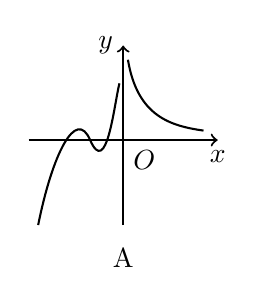
\begin{tikzpicture}[line width=0.75pt,scale=0.6]
  \draw [->](-2,0)--(2,0)node[below]{$x$};
  \draw [->](0,-1.8)--(0,2)node[left]{$y$};
  \node at (0,0) [below right]{$O$};
  \draw[yshift=-0.3cm] (-1.8,-1.5)..controls (-1.5,0) and (-1,1)..(-0.7,0.3)..controls(-.35,-0.5) and (-.2,1)..(-0.08,1.5);
  \draw (0.1,1.7)..controls (0.3,0.5) and (1,0.3)..(1.7,0.2);
  \node at (0,-2.5){A};
  \end{tikzpicture}
  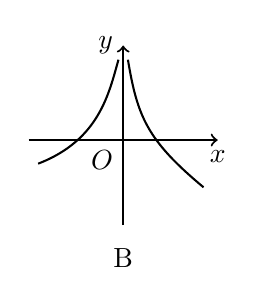
\begin{tikzpicture}[line width=0.75pt,scale=0.6]
  \draw [->](-2,0)--(2,0)node[below]{$x$};
  \draw [->](0,-1.8)--(0,2)node[left]{$y$};
  \node at (0,0) [below left]{$O$};
  \draw (-1.8,-0.5)..controls (-0.5,0) and (-0.3,1)..(-0.1,1.7);
  \draw (0.1,1.7)..controls (0.3,0.5) and (0.5,0)..(1.7,-1);
  \node at (0,-2.5){B};
  \end{tikzpicture}
  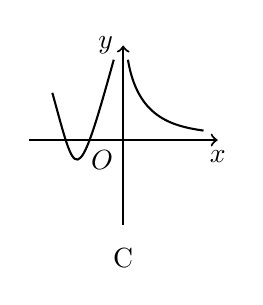
\begin{tikzpicture}[line width=0.75pt,scale=0.6]
  \draw [->](-2,0)--(2,0)node[below]{$x$};
  \draw [->](0,-1.8)--(0,2)node[left]{$y$};
  \node at (0,0) [below left]{$O$};
  \draw (-1.5,1)..controls (-1,-0.8) and (-1,-1.2)..(-0.2,1.7);
  \draw (0.1,1.7)..controls (0.3,0.5) and (1,0.3)..(1.7,0.2);
  \node at (0,-2.5){C};
  \end{tikzpicture}
  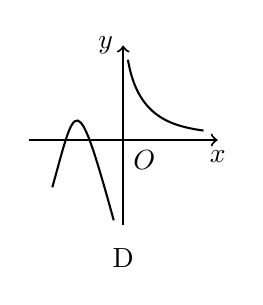
\begin{tikzpicture}[line width=0.75pt,scale=0.6]
  \draw [->](-2,0)--(2,0)node[below]{$x$};
  \draw [->](0,-1.8)--(0,2)node[left]{$y$};
  \node at (0,0) [below right]{$O$};
  \draw (-1.5,-1)..controls (-1,0.8) and (-1,1.2)..(-0.2,-1.7);
  \draw (0.1,1.7)..controls (0.3,0.5) and (1,0.3)..(1.7,0.2);
  \node at (0,-2.5){D};
  \end{tikzpicture}\qquad
\begin{tikzpicture}[line width=0.75pt,scale=0.6]
  \draw [->](-2,0)--(2,0)node[below]{$x$};
  \draw [->](0,-1.8)--(0,2)node[left]{$y$};
  \node at (0,0) [below left]{$O$};
  \draw (-1.8,-0.5)..controls (-1.5,0.3) and (-1,0.8)..(-0.5,0)..controls (-0.2,0.5) and (-0.1,1)..(-0.1,1.5);
  \draw (0.3,-1.8)..controls (.3,-1) and (0.8,0.8)..(1.6,1.7);
  \node at (0,-2.5){图1};
  \end{tikzpicture}





\item 观察下列各等式:$5^5=3125,5^6=15625,5^7=78125,\cdots$,则$5^{2013}$的末四位数是
  \fourch{3125} {5625} {8125}{0625}

\item 已知下列命题:

\cmcirc{1}$\sqrt7-\sqrt5\le\sqrt{10}-\sqrt2$;

\cmcirc{2}$\triangle ABC$的三个内角满足$\sin A+\sin B>\sin C$;

\cmcirc{3}存在等比数列$\{a_n\}$满足$a_1+a_3=2a_2$成立.

其中所有正确的命题序号是
  \fourch{{\cmcirc{1}}}{{\cmcirc{1} \cmcirc{2}}}{{\cmcirc{2}\cmcirc{3}}}{{\cmcirc{1} \cmcirc{2} \cmcirc{3}}}


\item 若水以恒速(即单位时间内注入的体积相同)注入图2的容器,则容器中的水的高度$h$ 与时间$t$ 的函数关系图象是(\qquad)

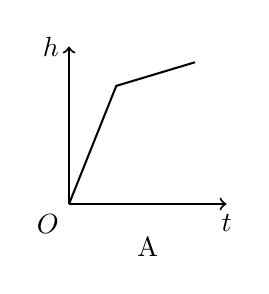
\begin{tikzpicture}[line width=0.75pt]
  \draw [->](0,0)--(2,0)node[below]{$t$};
  \draw [->](0,0)--(0,2)node[left]{$h$};
  \node at (0,0) [below left]{$O$};
  \draw(0,0)-- (0.6,1.5)--(1.6,1.8);
  \node at (1,-.3) [below]{A};
  \end{tikzpicture}
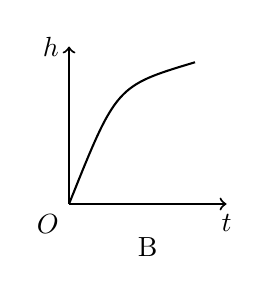
\begin{tikzpicture}[line width=0.75pt]
\draw [->](0,0)--(2,0)node[below]{$t$};
\draw [->](0,0)--(0,2)node[left]{$h$};
\node at (0,0) [below left]{$O$};
\draw(0,0).. controls(0.6,1.5)..(1.6,1.8);
  \node at (1,-.3) [below]{B};
 \end{tikzpicture}
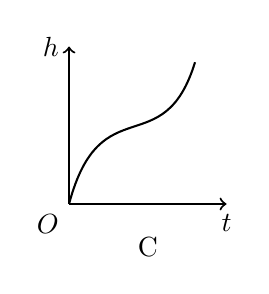
\begin{tikzpicture}[line width=0.75pt]
 \draw [->](0,0)--(2,0)node[below]{$t$};
\draw [->](0,0)--(0,2)node[left]{$h$};
\node at (0,0) [below left]{$O$};
\draw(0,0).. controls(0.4,1.5)and(1.2,0.5)..(1.6,1.8);
  \node at (1,-.3) [below]{C};
\end{tikzpicture}
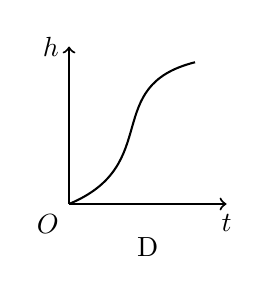
\begin{tikzpicture}[line width=0.75pt]
\draw [->](0,0)--(2,0)node[below]{$t$};
\draw [->](0,0)--(0,2)node[left]{$h$};
\node at (0,0) [below left]{$O$};
\draw(0,0).. controls(1.2,0.5)and(0.4,1.5)..(1.6,1.8);
  \node at (1,-.3) [below]{D};
\end{tikzpicture}
\begin{tikzpicture}[line width=0.75pt,yscale=0.618]
 \draw(-1.8,-1.2)(0,0);   %这是纯粹将图片抬高,以使与版面匹配,开始没统筹好
 \draw(1,0)--(1.4,1)--(1,2)(0,2)--(-0.4,1)--(0,0);
 \draw(0,0) arc (-180:0:0.5 and 0.2);
 \draw[dashed](1,0) arc (0:180:0.5 and 0.2);
 \draw(-0.4,1) arc (-180:0:0.9 and 0.36);
 \draw[dashed](1.4,1) arc (0:180:0.9 and 0.36);
 \draw(-0.4,1) arc (-180:0:0.9 and 0.36);
 \draw[dashed](1.4,1) arc (0:180:0.9 and 0.36);
 \draw(0.5,2) ellipse (0.5 and 0.2);
 \node at (0.5,-0.5) [below]{图2};
 \end{tikzpicture}





\item 若函数$f(x)=x^3+ax+b$有三个零点,分别为$x_1,x_2,x_3$,且满足$x_1<1,x_2=1,x_3>1$,则实数$a$ 的取值范围是
    \fourch{$(-\infty,0)$}{$(-\infty,-1)$}{$(-\infty,-2)$}{$(-\infty,-3)$}



\item 已知正方体$ABCD-A_1B_1C_1D_1$的棱长为1,如图3,$P$是截面$A_1BD$内(包括边界)的动点,则${\vv {C_1P}\cdot \vv {C_1B}}$ 的值不可能是
\fourch{0.9}{1.2}{1.5}{1.8}
\begin{center}
 \begin{tikzpicture}[line width=0.75,scale=2.5]
      \coordinate (A) at (0, 0);
         \coordinate (B) at (1, 0);
           \coordinate (C) at (1.3, 0.3);
             \coordinate (D) at (0.3, 0.3);
               \coordinate (A1) at (0, 1);
                 \coordinate (B1) at (1, 1);
                   \coordinate (C1) at (1.3, 1.3);
                     \coordinate (D1) at (0.3, 1.3);
       \node  at (A)[left]{$A$};
         \node  at (B)[right]{$B$};
            \node  at (C)[right]{$C$};
               \node at (D)[left]{$D$};
             \node  at (D1)[left]{$D_1$};
          \node  at (C1)[right]{$C_1$};
        \node  at (B1)[below right]{$B_1$};
      \node at (A1)[left]{$A_1$};

  \draw (A)--(B)--(C)--(C1)--(B1)--(A1)--(A)(A1)--(D1)--(C1)(B1)--(B)(A1)--(B);
  \draw [dashed](D)--(A)(D)--(C)(D)--(D1)(D)--(B)(D)--(A1)(C1)--(0.36,0.5);
  \node at (0.36,0.5)[below]{$P$};
   \node at (0.5,0)[below=1pt]{图3};
   \end{tikzpicture}\hfill
   \begin{tikzpicture}[line width=0.75,scale=2.5]
      \coordinate (A) at (0, 0);
         \coordinate (B) at (1, 0.3);
           \coordinate (C) at (-0.3,0.3);
              \coordinate (A1) at (0, 1);
                 \coordinate (B1) at (1, 1.3);
                   \coordinate (C1) at (-0.3, 1.3);
                \node  at (A)[left]{$A$};
             \node  at (B)[right]{$B$};
          \node  at (C)[left]{$C$};
       \node  at (C1)[left]{$C'$};
     \node  at (B1)[above]{$B'$};
  \node at (A1)[below right]{$A'$};
     \coordinate (E) at (0.5, 1.15);
       \node at (E)[below]{$E$};
  \draw (A)--(B)--(B1)--(A1)--(C1)--(B1)(A1)--(A)--(C)--(C1);
  \draw [dashed](C)--(B)(C)--(E);
  \node at (0.35,0)[below=1pt]{图4};
   \end{tikzpicture}

\end{center}

\end{enumerate}

\end{itemize}


\begin{itemize}
\item[\Heiti 二.] {\Heiti  填空题:本大题共6小题,第小题4分,共24分.把答案填在题中横线上}


 \linespread{2.2}\selectfont\begin{enumerate}[leftmargin=*]\addtocounter{enumi}{8}

\item 已知三个点$A(1,-1,b),B(2,a,1),O(0,0,0)$在同一条直线上,\\则$a=$\hhh,$b=$\hhh.

\item 若函数$y=ax-\sin x$是$\mathbb{R}$上的单调递增函数,则实数$a$的取值范围\hhh.

\item 由曲线$y=x^2$和直线$y=2x$围成的封闭区域的面积为\hhh.


\item 如图4所示,已知三棱柱$A'B'C'-ABC$的侧棱垂直于底面,$AC \perp CB$,且$AC=CB=CC'=2$. 若$E$为$A'B'$ 中点,则$CE$ 与底面$ABC$所成角的余弦值为\hhh.

\item 若函数$f(x)=(x^2-3)\mathrm{e}^x$,给出下面四个结论:

\cmcirc{1}$f(-3)$是$f(x)$的极大值,$f(1)$是$f(x)$的极小值;

\cmcirc{2}$f(0)<0$的解集为$\{x|-\sqrt x < x< \sqrt 3\}$;

\cmcirc{3}$f(x)$没有最小值,也没有最大值;

\cmcirc{4}$f(x)$ 有最小值,没有最大值.

其中正确的结论序号有\hhh.


\item 已知函数$f(x)=\dfrac x{x+3}$,构造如下函数序列$f_n(x):f_n(x)=f[f_{n-1}(x)](n\in \mathbb{N}^*,\text{且}n\ge 2)$,其中$f_1(x)=f(x),(x>0)$,则$f_3(x)=$\hhh, 函数$f_n(x)$ 的值域为\hhh[2].



\end{enumerate}

\end{itemize}



\begin{itemize}
\item[\Heiti 三.]{\Heiti 解答题,本大题共4小题,共44分.解答应写出文字说明,证明过程或演算步骤}
\begin{enumerate}[leftmargin=*]\addtocounter{enumi}{14}

\item (本小题共10分)

已知函数$f(x)=\dfrac {a^2}3 x^3-2ax^2+bx$,其中$a,b\in \mathbb{R}$,且曲线$y=f(x)$在点$(0,f(0))$ 处的切线斜率为3.\begin{enumerate}[align=left,leftmargin=*,labelsep=0pt,label= \hspace{-0.33em} (\Roman*)]
                   \item 求$b$的值;
                   \item 若函数在$x=1$处取得极大值,求$a$的值.
        \end{enumerate}

\vfill

\item (本小题共10分)

已知点列$A_n(x_n,0),n\in \mathbb{N}^*$,其中$x_1=0,x_2=a(a>0)$,$A_3$是线段$A_1A_2$的中点,$A_4$是线段$A_2A_3$的中点,$\cdots A_n$是线段$A_{n-2}A_{n-1}$的中点,$\cdots$.\begin{enumerate}[align=left,leftmargin=*,labelsep=0pt,label= \hspace{-0.33em} (\Roman*)]
                   \item 写出$x_n,x_{n-1},x_{n-2}$之间的关系式$(n\ge 3)$;
                   \item 设$a_n=x_{n+1}-x_n$,计算$a_1,a_2,a_3$的值,由此推测数列$\{a_n\}$的通项公式,并加以证明.
        \end{enumerate}
\vfill
\newpage
%\item  已知函数$f(x)=x^3-ax^2+bx+c$在$x=0$处取得\emph {极大值}1. 求实数$b,c$ 的值,并求实数$a$ 的取值范围.


\item (本小题共12分)

已知平面$ADEF\perp\text{平面}ABCD$,其中$ADEF$为矩形,$AB\sslash CD,AB\perp AD$,且$AB=2CD=2DE=4,AD=2\sqrt{2}$,如图5所示.\begin{enumerate}[align=left,leftmargin=*,labelsep=0pt,label= \hspace{-0.33em} (\Roman*)]
    \item 求证$BF\perp AC $;
    \item 求二面角$B-CE-D$的的余弦值;
    \item 在线段$AF$上是否存在点$P$,使得$BP\sslash \text{平面}ACE$,若存在,确定点$P$的位置.若不存在,请说明理由.\end{enumerate}

\hfill   \begin{tikzpicture}[line width=0.75,scale=2]
      \coordinate (A) at (0, 0);
         \coordinate (B) at (-1, -1);
           \coordinate (C) at (1.5,-0.5);
            \coordinate (D) at (2,0);
              \coordinate (E) at (2, 1);
                 \coordinate (F) at (0, 1);
                   \coordinate (P) at (0, 0.75);
                \node  at (A)[above left]{$A$};
             \node  at (B)[below]{$B$};
          \node  at (C)[right]{$C$};
       \node  at (D)[below right]{$D$};
     \node  at (E)[above]{$E$};
  \node at (F)[above]{$F$};
   \node at (P)[below right]{$P$};
  \draw (A)--(B)--(C)--(D)--(E)--(F)--(A)--(E)(P)--(B)--(E)--(C);
  \draw [dashed](A)--(C)(A)--(D);
  \node at (0.6,-1)[below=1pt]{图5};
\end{tikzpicture}
\vfill


\item (本小题共12分)

已知函数$f(x)=ax^2-(a+1)x+\ln x$.\begin{enumerate}[align=left,leftmargin=*,labelsep=0pt,label= \hspace{-0.33em} (\Roman*)]
    \item 当$a=-2$时,判断函数$f(x)$零点的个数;
    \item 求函数$f(x)$的单调区间.\end{enumerate}
\vfill
\end{enumerate}

\end{itemize}

\end{document}
